% Figuras reproducibles: scripts/figuras_cuerpo.py. Las tablas del anexo se conservan.
Las Figuras~\ref{fig:contexto-edad} a~\ref{fig:contexto-region} presentan el corte 28 como ejemplo de lectura de las categorías; esta elección no establece que sea el mejor momento para predecir. En ese corte se incluyen 27\,515 inscripciones elegibles y se observan 5\,012 retiros posteriores, equivalentes al 18,2\%. Cada barra expresa el porcentaje dentro de su categoría y la línea discontinua señala el porcentaje general. Los conteos completos de los cinco cortes permanecen en el Anexo~\ref{corr:anexocontexto}, Tabla~\ref{corr:niveles}.

\Needspace{.40\textheight}\subsection{Edad y discapacidad registrada}
La Figura~\ref{fig:contexto-edad} permite comparar los porcentajes de retiro sin perder de vista el tamaño de cada grupo. La categoría de 55 o más años reúne solo 193 inscripciones, frente a 19\,166 en la primera banda. Por ello, los porcentajes deben leerse junto con sus denominadores; el menor porcentaje observado en un grupo pequeño no demuestra una ventaja general asociada con la edad. Se conservan las bandas definidas por OULAD.
\begin{figure}[H]\centering
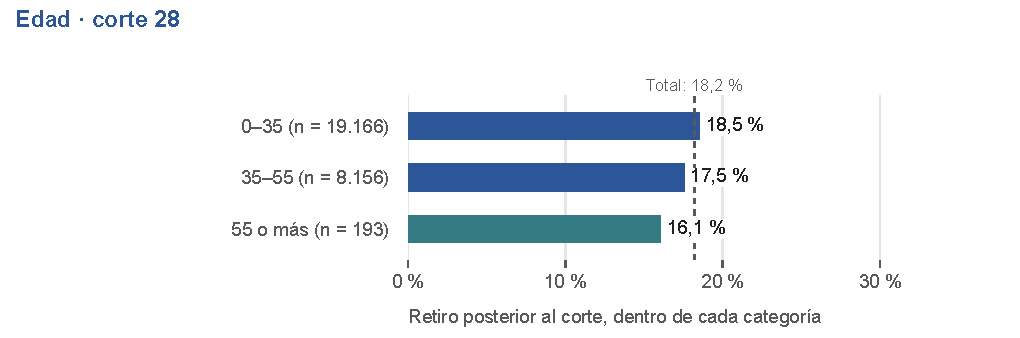
\includegraphics[width=\linewidth]{figuras_contexto/contexto_age_band_28.pdf}
\caption[Retiro futuro por banda de edad al día 28.]{Retiro futuro por banda de edad al día 28. $n$ indica inscripciones de cada categoría. Elaboración propia a partir de los conteos de la Tabla~\ref{corr:niveles} del anexo.}\label{fig:contexto-edad}
\end{figure}

La Figura~\ref{fig:contexto-discapacidad} muestra un porcentaje observado de 26,0\% entre las inscripciones con discapacidad registrada y de 17,4\% entre aquellas sin ese registro afirmativo. La diferencia descriptiva es de 8,6 puntos porcentuales. Esta comparación no ajusta por módulo, calendario u otras características y no identifica la causa de la diferencia.
\begin{figure}[H]\centering
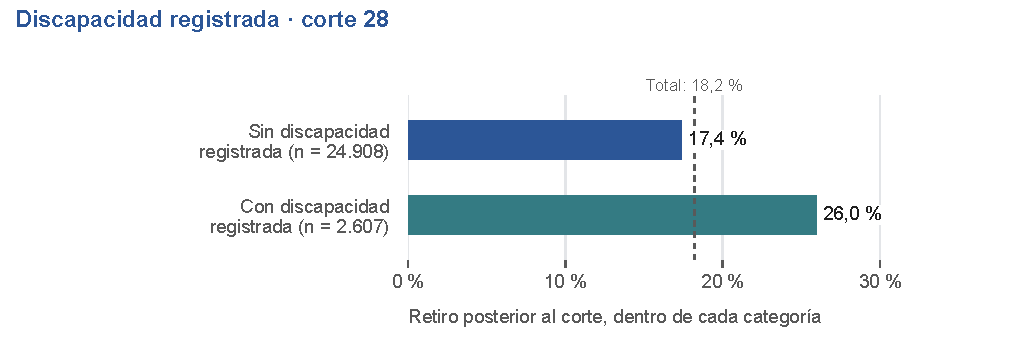
\includegraphics[width=\linewidth]{figuras_contexto/contexto_disability_28.pdf}
\caption[Retiro futuro según discapacidad registrada al día 28.]{Retiro futuro según discapacidad registrada al día 28. Los tamaños de los grupos se muestran junto a las etiquetas. Elaboración propia; conteos en la Tabla~\ref{corr:niveles} del anexo.}\label{fig:contexto-discapacidad}
\end{figure}

\subsection{Privación del área de residencia y región}
Las bandas de IMD se mantienen en su orden original en la Figura~\ref{fig:contexto-imd}. Los porcentajes oscilan entre bandas y no siguen una disminución uniforme. Los casos sin dato se muestran en gris: corresponden a 1\,027 inscripciones y no deben interpretarse como una banda adicional de privación. La figura describe diferencias entre grupos de áreas de residencia, sin trasladar automáticamente esa interpretación a los recursos económicos de cada persona.
\begin{figure}[H]\centering
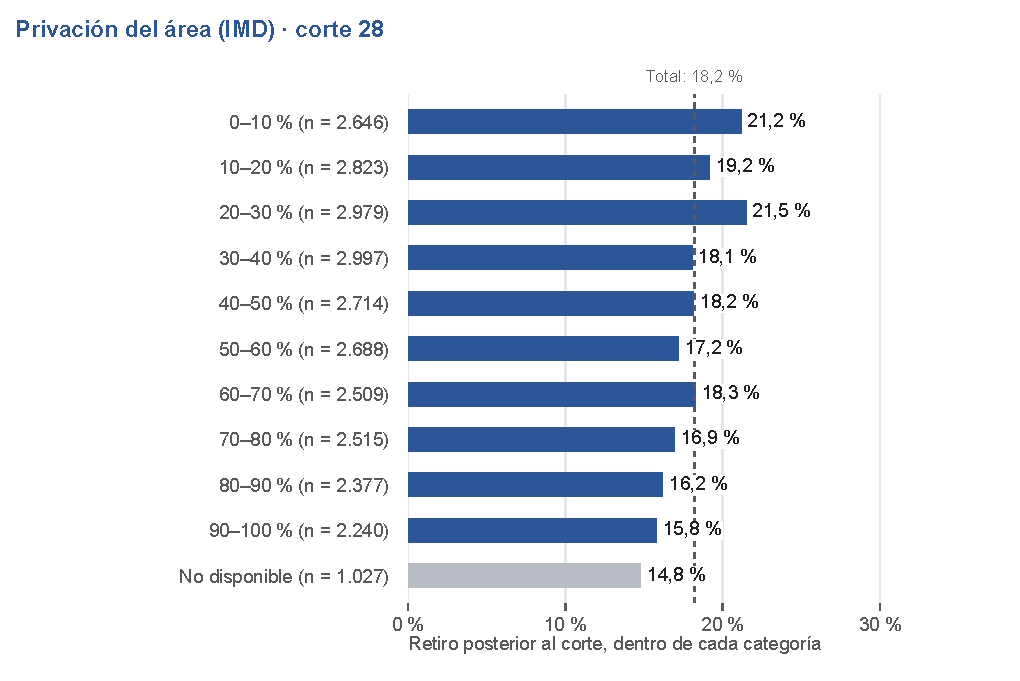
\includegraphics[width=\linewidth]{figuras_contexto/contexto_imd_band_28.pdf}
\caption[Retiro futuro por banda de IMD al día 28.]{Retiro futuro por banda de IMD al día 28. La línea discontinua representa el porcentaje general del corte. Elaboración propia; valores y denominadores en la Tabla~\ref{corr:niveles} del anexo.}\label{fig:contexto-imd}
\end{figure}

En la Figura~\ref{fig:contexto-region}, las regiones se ordenan por su porcentaje observado para facilitar la comparación. El rango va de 16,7\% en East Anglian Region a 19,8\% en West Midlands Region. Este orden resume el corte 28 y no constituye una clasificación permanente de las regiones ni una comparación ajustada de sus condiciones educativas.
\begin{figure}[H]\centering
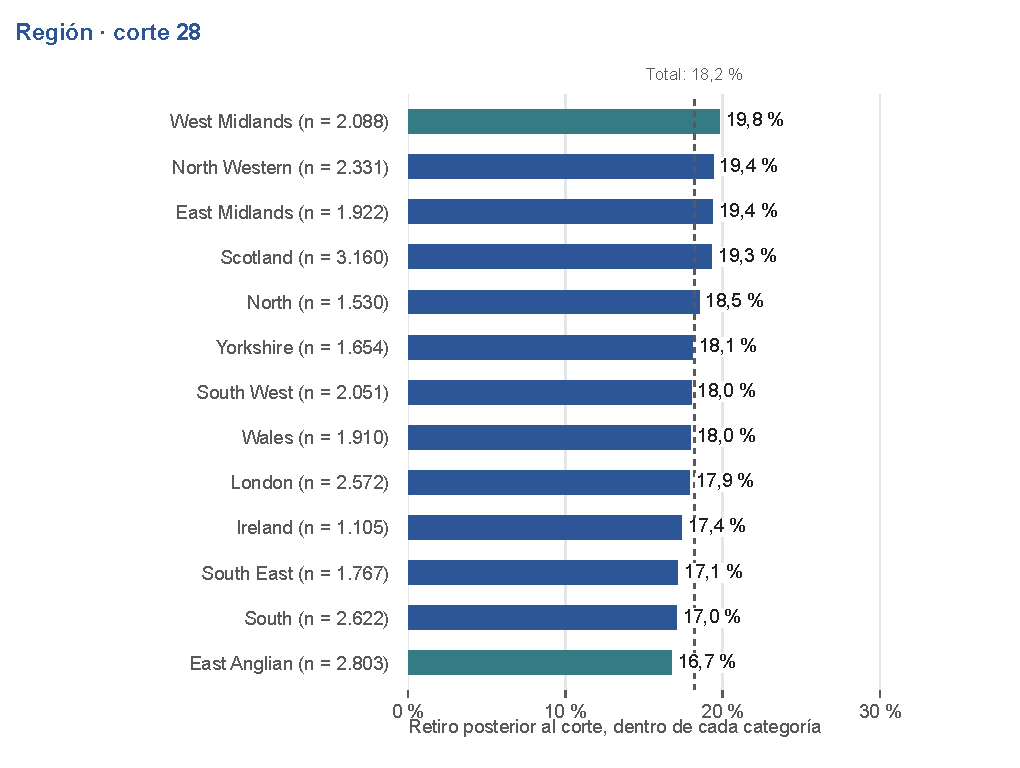
\includegraphics[width=\linewidth]{figuras_contexto/contexto_region_28.pdf}
\caption[Retiro futuro por región al día 28.]{Retiro futuro por región al día 28. Se abrevia la palabra \textit{Region} en las etiquetas. Elaboración propia; conteos completos en la Tabla~\ref{corr:niveles} del anexo.}\label{fig:contexto-region}
\end{figure}

\subsection{Lectura conjunta de los cinco cortes}
Las Figuras~\ref{fig:contexto-cortes} y~\ref{fig:contexto-region-cortes} reúnen los porcentajes de los cinco cortes mediante una escala común: un azul más oscuro representa un porcentaje mayor. Cada columna identifica su población elegible. La lectura horizontal describe cómo cambian los porcentajes publicados, pero no sigue una población fija: entre cortes cambian las inscripciones incluidas y el tiempo restante hasta el final del curso. Por ello, una reducción del porcentaje no demuestra una mejora predictiva ni una disminución del riesgo de una misma persona.
\begin{figure}[H]\centering
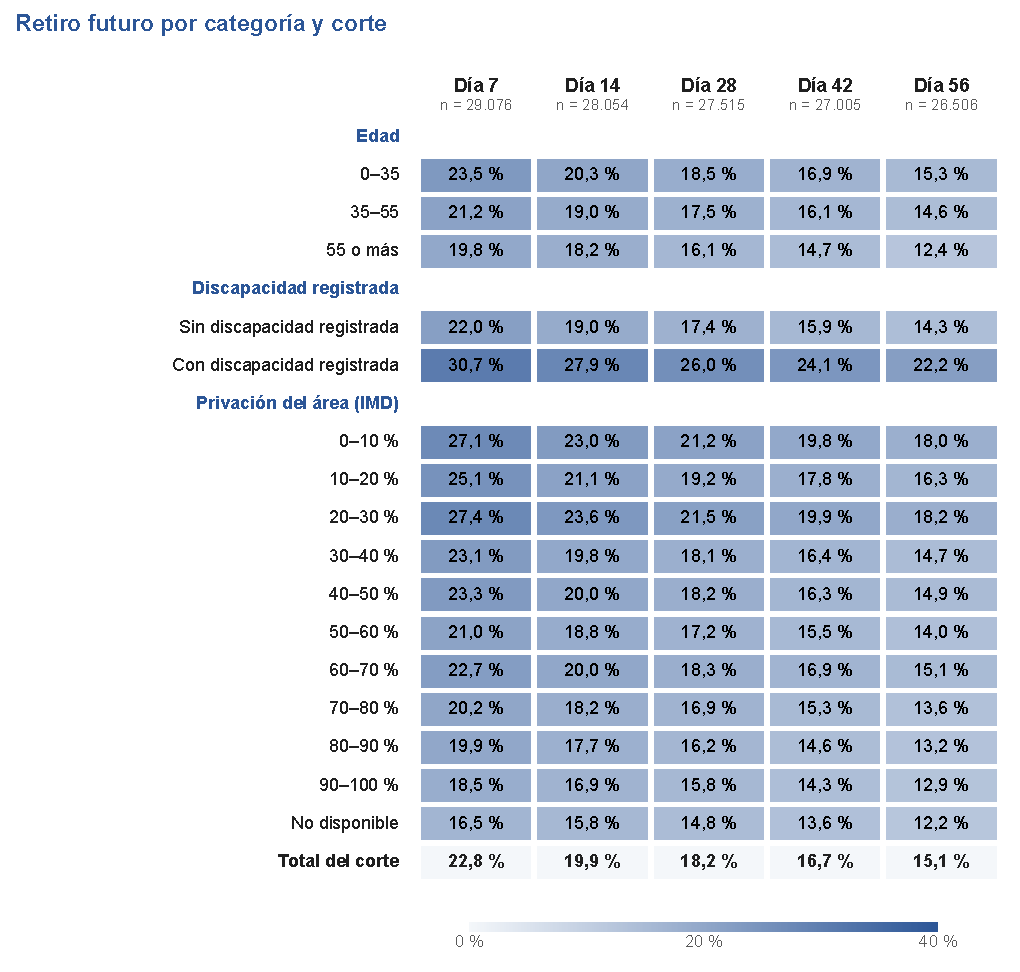
\includegraphics[width=\linewidth]{figuras_contexto/contexto_cortes.pdf}
\caption[Retiro futuro por edad, discapacidad e IMD en cinco cortes.]{Retiro futuro por edad, discapacidad registrada e IMD en los cinco cortes. La fila final muestra el porcentaje general de cada corte. Elaboración propia; numeradores y denominadores por categoría en la Tabla~\ref{corr:niveles} del anexo.}\label{fig:contexto-cortes}
\end{figure}

La Figura~\ref{fig:contexto-region-cortes} conserva el mismo orden alfabético de las regiones en todas las columnas. Esta disposición permite localizar cada región sin confundir un cambio en el orden de las filas con un cambio en los resultados. Los valores corresponden al retiro registrado después de cada corte y hasta el final del curso.
\begin{figure}[H]\centering
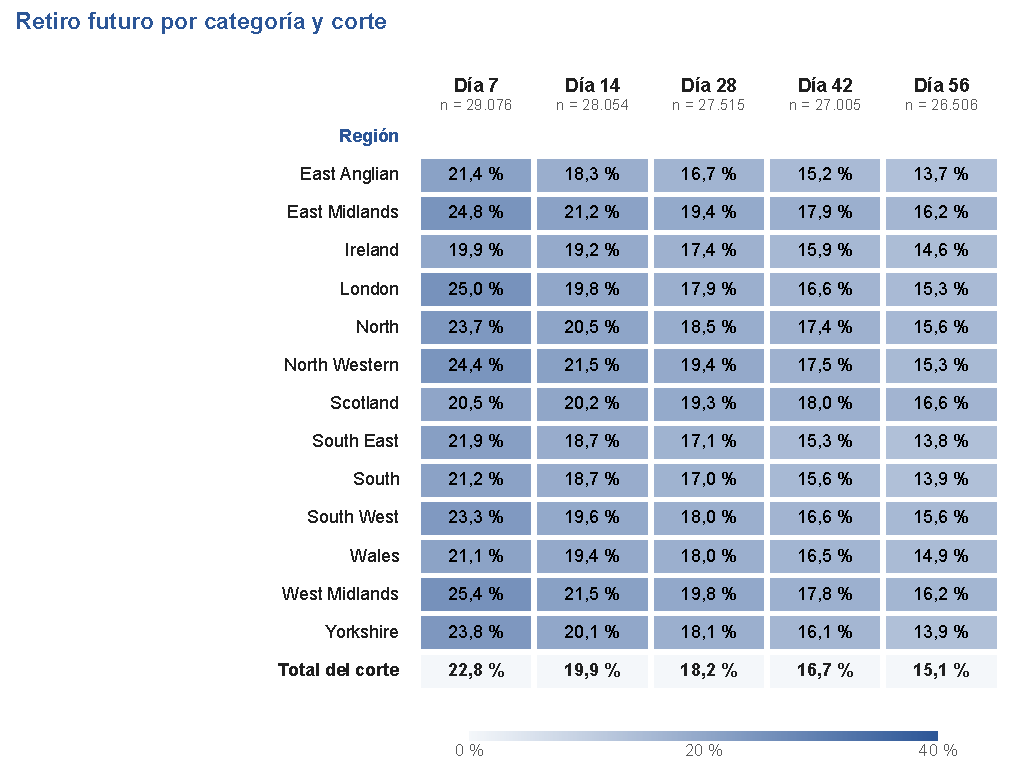
\includegraphics[width=\linewidth]{figuras_contexto/contexto_region_cortes.pdf}
\caption[Retiro futuro por región en cinco cortes.]{Retiro futuro por región en los cinco cortes. Se utiliza la misma escala de color que en la Figura~\ref{fig:contexto-cortes}. Elaboración propia; detalle en la Tabla~\ref{corr:niveles} del anexo.}\label{fig:contexto-region-cortes}
\end{figure}

\Needspace{.42\textheight}\subsection{Créditos e intentos previos}
